\documentclass{beamer}
\usepackage{tikz}
\usepackage{graphicx}
\usetikzlibrary{positioning}
\usetikzlibrary{calc}
%\usetikzlibrary{arrows}

\usefonttheme{professionalfonts}
\usetheme{Boadilla}
\setbeamertemplate{navigation symbols}{}%remove navigation symbols
\hypersetup{pdfstartview={Fit}} % fits the presentation to the window when first displayed
\graphicspath{{./figures/}{./figures/generated/}{./figures/static/}}

%Edwards PB, Wanjura WJ, Brown WV: Selective herbivory by Christmas beetles in response to intraspecific variation in Eucalyptus terpenoids. Oecologia 1993, 95:551–557

%Info
\title[Detecting Somatic Mutations]{Methods for Detecting Somatic Mutation in Plants}
\titlegraphic{
	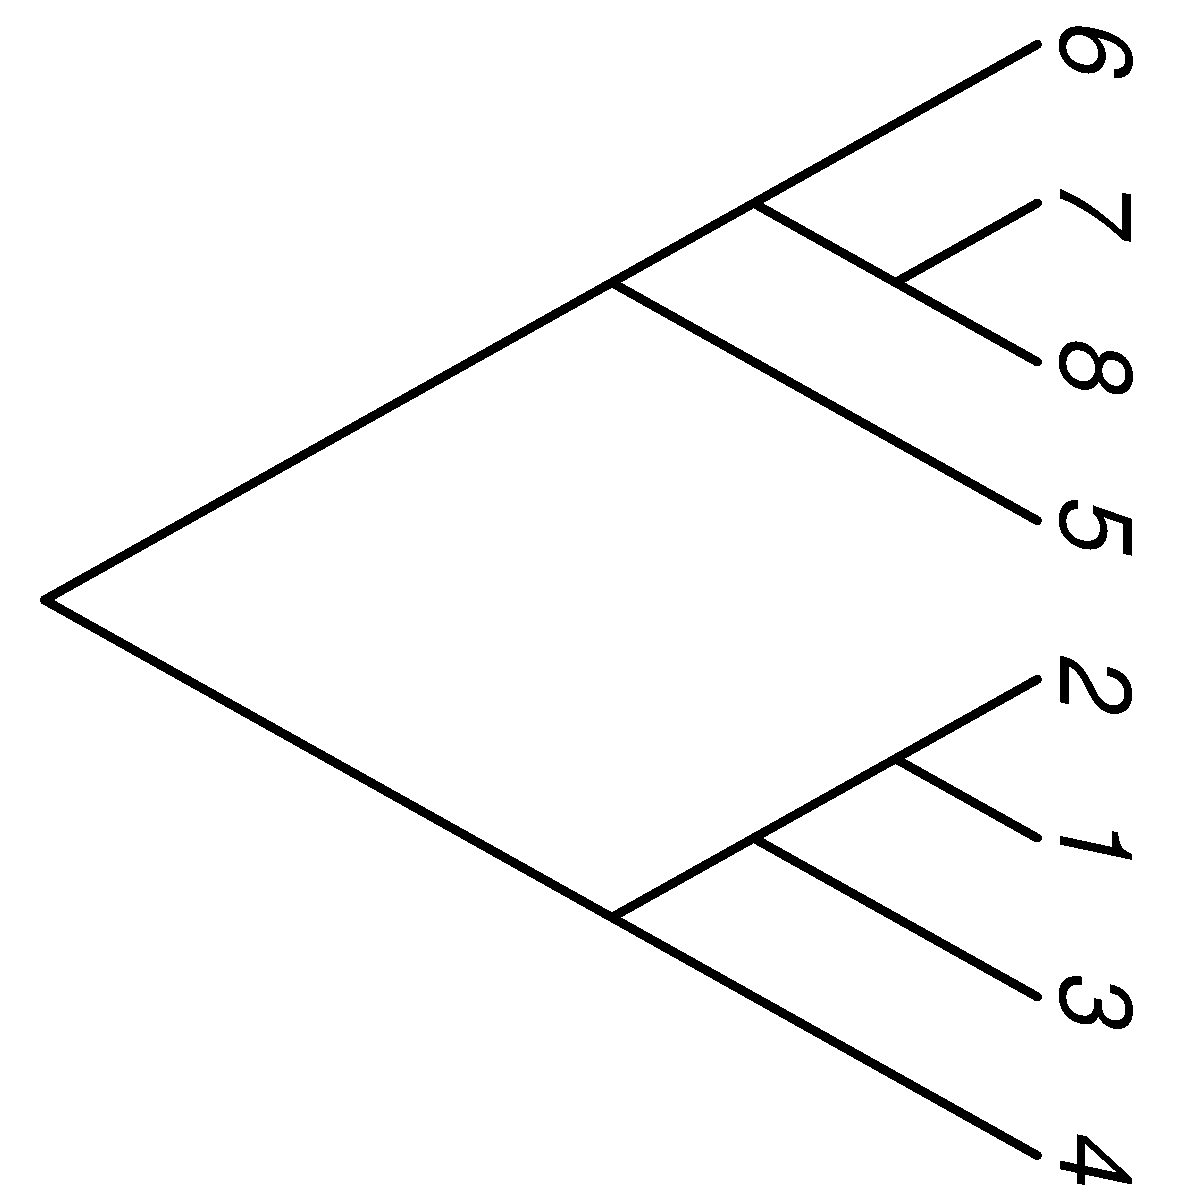
\includegraphics[width=.3\linewidth]{gatk_tree_rightwards.pdf}
	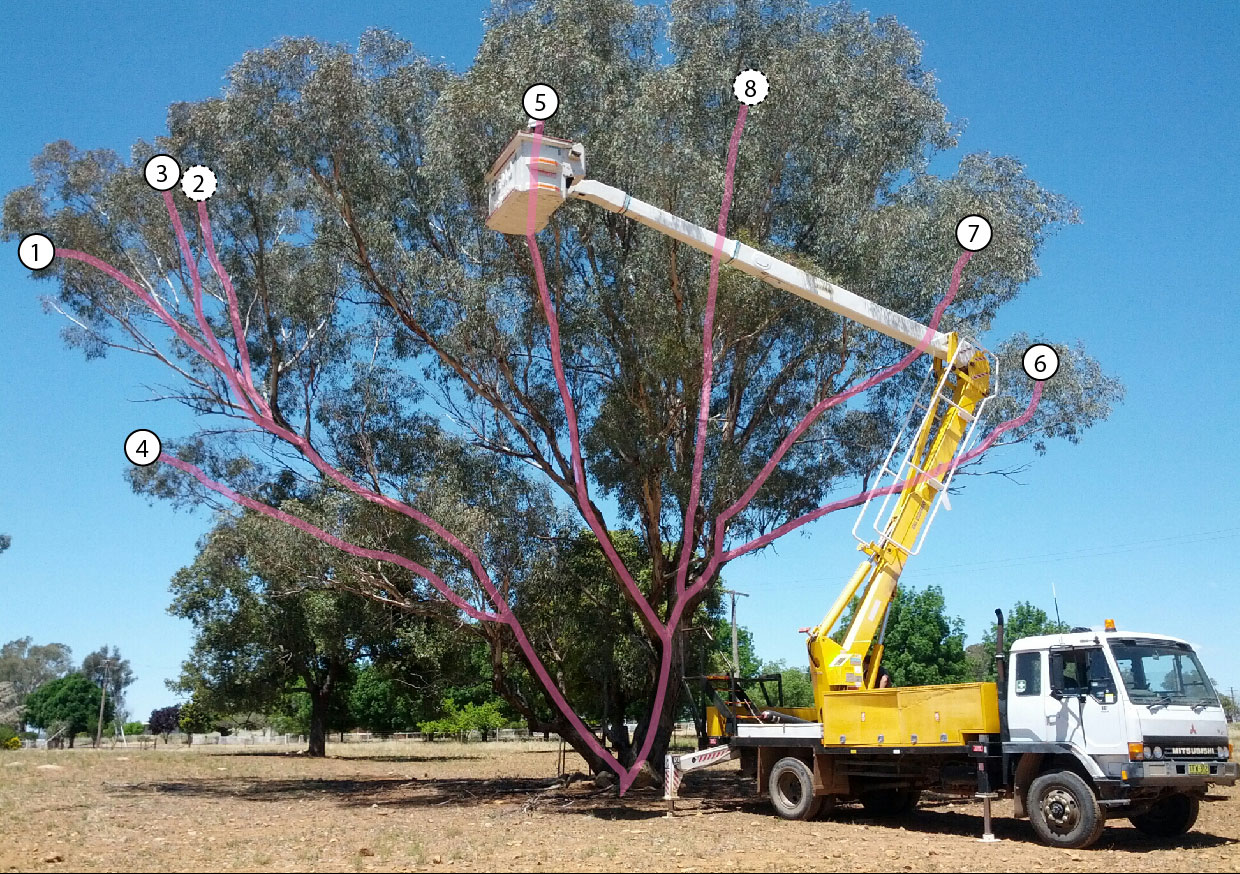
\includegraphics[width=.3\textwidth, angle=90]{labeled_tree.jpg}
	}
\date{5/02/17}
\author{Adam Orr}

\begin{document}
\frame{\titlepage}
\begin{frame}{The Yellow Box Tree: \textit{Eucalyptus melliodora}}

\begin{columns}
\column{.5\linewidth}
\begin{itemize}
\item Produces \textbf{5 times} more nectar than smaller trees.
\item Food source for bees
\item Strong wood used for bridges
\end{itemize}
\column{.5\linewidth}
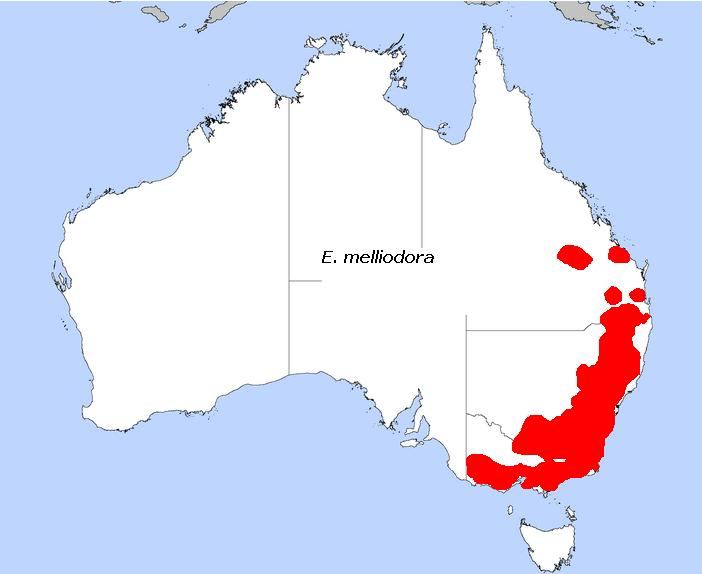
\includegraphics[width=\linewidth]{map.jpg}\footnotemark
\end{columns}
\footnotetext{\url{https://commons.wikimedia.org/wiki/File:E._melliodora.JPG}}
\end{frame}

\begin{frame}{A Genetic Mosaic}
	\begin{center}
	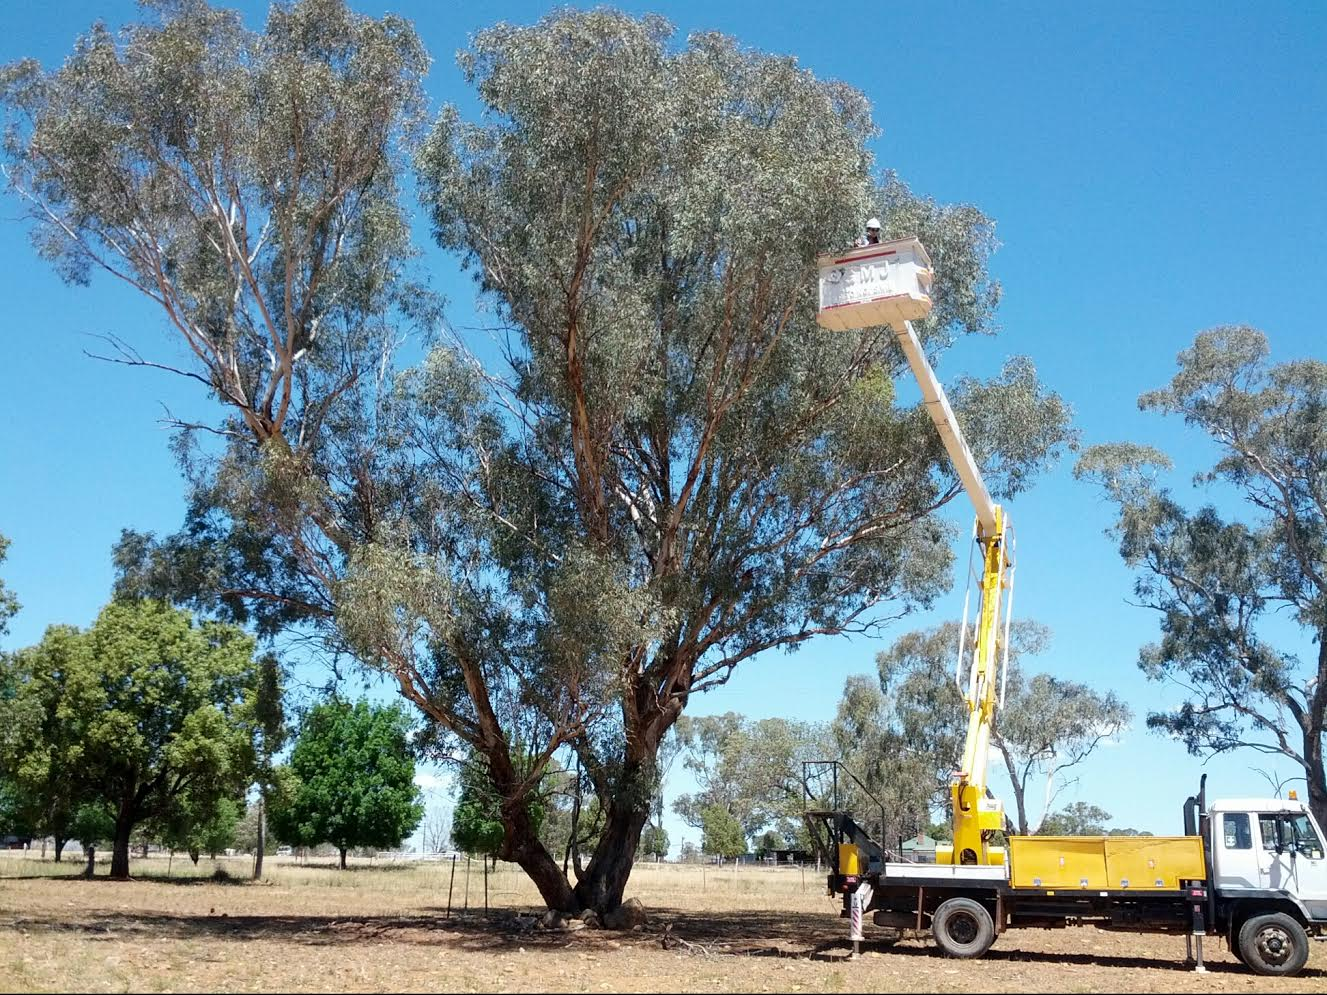
\includegraphics[width=.6\linewidth]{unlabeled_tree.jpg}
	\end{center}
	\begin{itemize}
		\item Edwards identified as mosaic in 1993\footnote{\textit{Edwards PB, Wanjura WJ, Brown WV. Oecologia 1993, 95:551–557.}}
		\item Sheep pen in Yeoval, New South Wales
		\item Differential oil production gives protection from Christmas beetles
		\item Is this mutation a controlled process?
	\end{itemize}
\end{frame}

\begin{frame}{Somatic Mutations are Commercially Interesting}
	\begin{definition}
		A \textbf{somatic mutation} is a mutation that occurs in non-germline cells	
	\end{definition}
	\begin{itemize}
		\item Nectarines arose from a somatic mutation on a peach tree %mosaicism in plants is commercially interesting, though we don't understand it
		\item In botany, this is called a \textbf{sport}
		\item Limited understanding of how plants grow
	\end{itemize}
	\begin{center}
	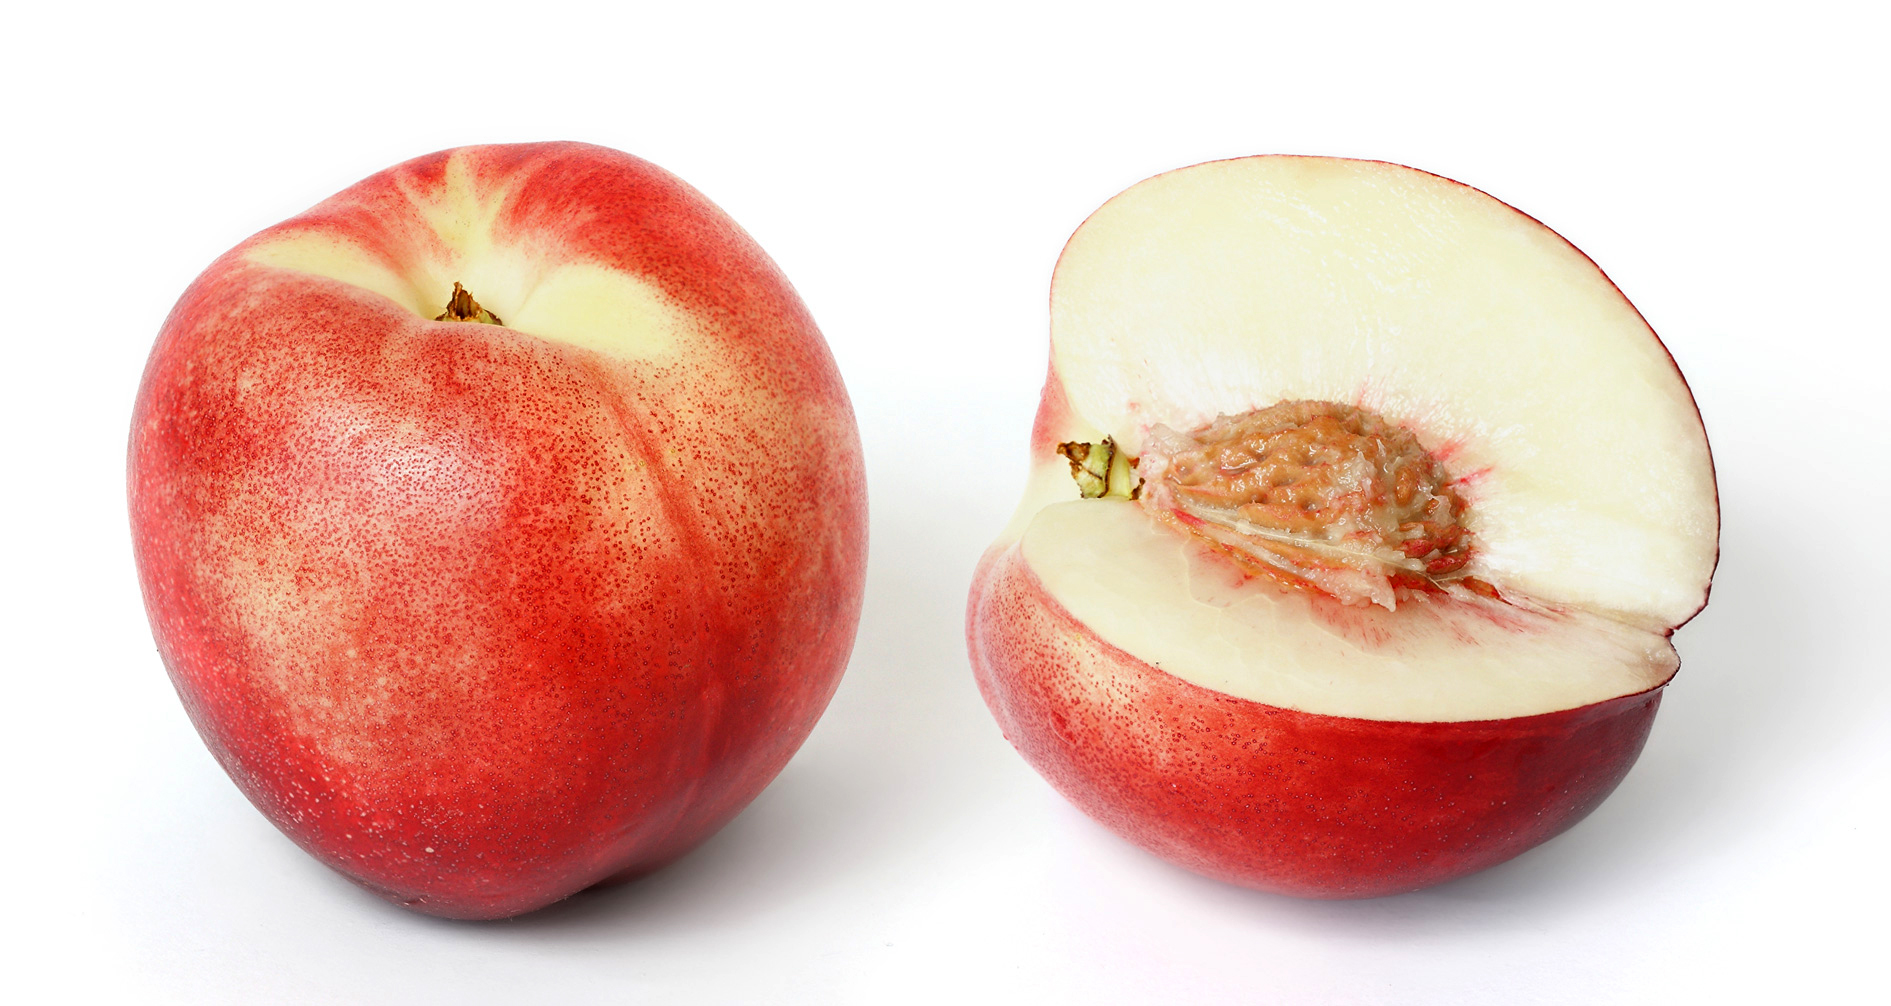
\includegraphics[width=.6\linewidth]{nectarine.jpg}
	\footnote{\url{https://commons.wikimedia.org/wiki/File:White_nectarine_and_cross_section02_edit.jpg}}
	\end{center}
\end{frame}

\begin{frame}{Broad Implications}
	\begin{itemize}
	\item How do somatic mutations spread? How can we study this?
	\item Cancers and other somatic diseases.
	\item A tree as a system for studying somatic mutation.
	\item The tree has a built-in control
	\end{itemize}

	% \begin{alertblock}{A phylogeny is a \textbf{hypothesis}!}
	% 	We use simulations because we can't know the truth \\~\\

	% 	Knowing the truth will allow us to evaluate phylogenetic tools		
	% \end{alertblock}

\end{frame}

\begin{frame}{What mutation is causing the herbivore resistance phenotype?}
\begin{center}
	\begin{tikzpicture}
		\node[anchor=south west,inner sep=0] (image) at (0,0) {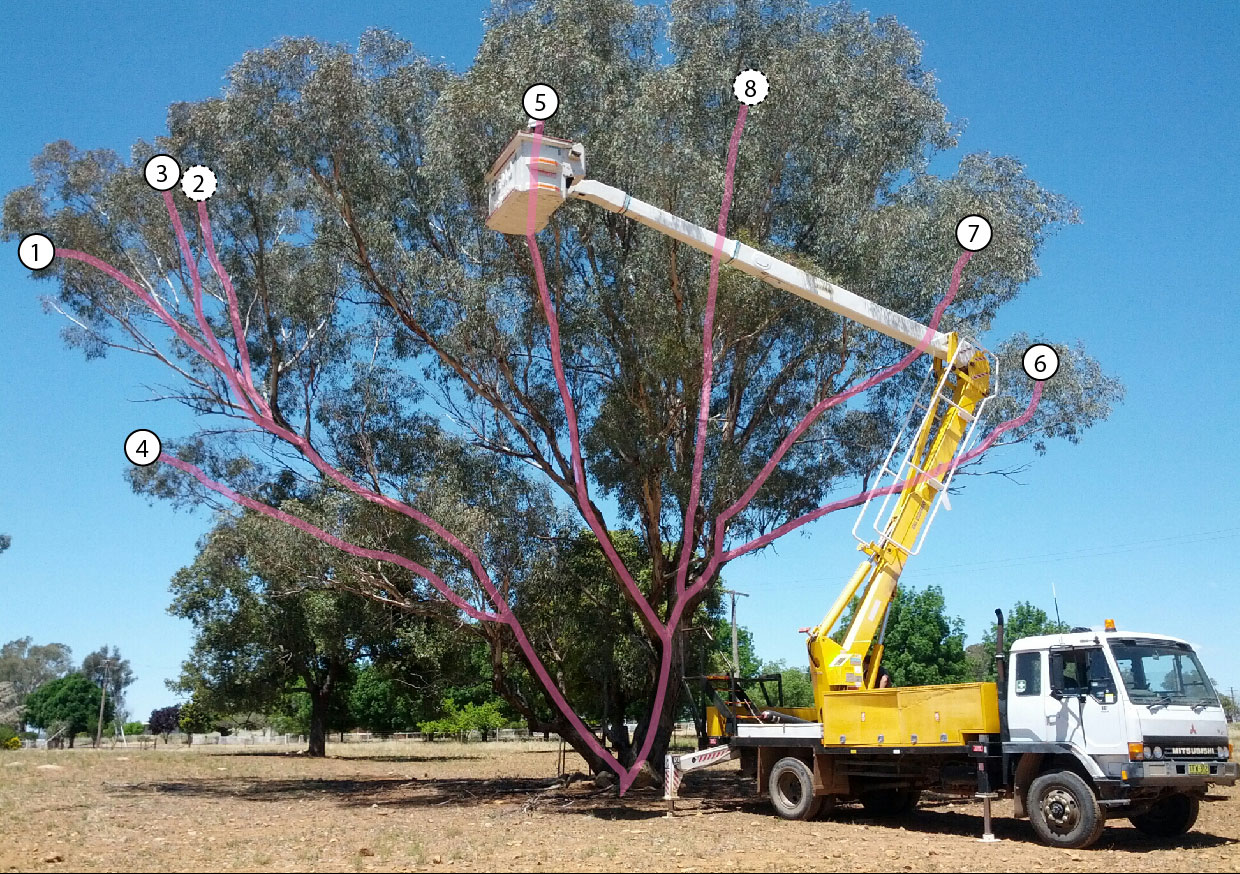
\includegraphics[width=\textwidth]{labeled_tree.jpg}};
		\begin{scope}[x={(image.south east)},y={(image.north west)}]
			\draw[red, line width=5mm, ->] (.35,.75) -- (.25,.5);
		\end{scope}
	\end{tikzpicture}
\end{center}
\end{frame}


%%A slide about cancer. Can we extract all the populations out of a tumor? Can we use a sequencing strategy to identify human GT vs cancer GT?

%%We believe it to be the case that flowers & reproductive cells are forming as the branch forms, not transported through a stem-cell store.

\begin{frame}{Mutations are very rare, but sequencing errors are very common.}

Somatic mutations are hard to find

\begin{itemize}
\item Errors accumulate during PCR prior to sequencing - then propagate
\item Errors accumulate in amplification steps during sequencing
\item Technical error from sequencer
\end{itemize}

\textbf{Sequencing error} alone is \textbf{$\sim10^{-2}$} while mutation rate after error-checking is \textbf{$\sim10^{-10}$}

\end{frame}

\begin{frame}{Study Methodology}
\begin{columns}

\column{.5\linewidth}
\begin{definition}
\textbf{Coverage:}Average number of times a single base is sequenced.
\end{definition}
\begin{itemize}
\item Sequence 8 samples in triplicate
\item Ultra-deep coverage for each replicate ($\sim$30X)
\item Align sequence to genome of \textit{Eucalyptus grandis}
\item Use replicates to remove false positives
\end{itemize}

\column{.5\linewidth}
\begin{center}
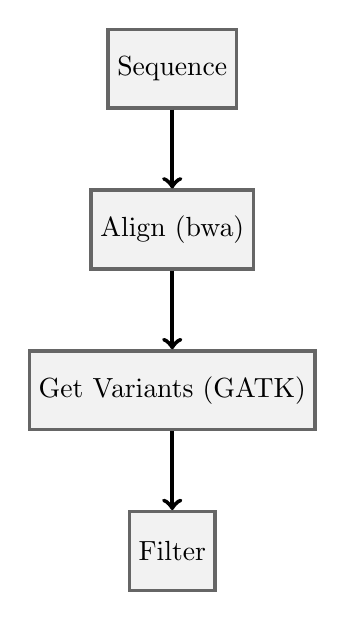
\begin{tikzpicture}[sqnode/.style={rectangle, draw=black!60, fill=black!5,very thick,minimum size=1cm}]
	\node[sqnode] (sequencing) {Sequence};
	\node[sqnode] (alignment) [below = of sequencing] {Align (bwa)};
	\node[sqnode] (varcall) [below = of alignment] {Get Variants (GATK)};
	\node[sqnode] (flt) [below = of varcall] {Filter};
	\draw[ultra thick,->] (sequencing.south) -- (alignment.north);
	\draw[ultra thick,->] (alignment.south) -- (varcall.north);
	\draw[ultra thick,->] (varcall.south) -- (flt.north);
\end{tikzpicture}
\end{center}
\end{columns}
\end{frame}

\begin{frame}{GATK Best Practices}
\begin{center}
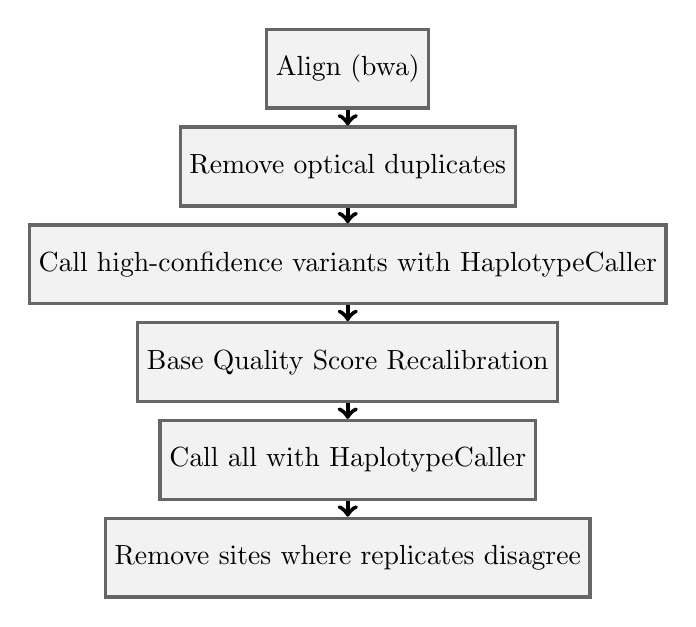
\begin{tikzpicture}[sqnode/.style={rectangle, draw=black!60, fill=black!5,very thick,minimum size=1cm}, node distance = .2cm]
	\node[sqnode] (alignment) {Align (bwa)};
	\node[sqnode] (deduplify) [below = of alignment] {Remove optical duplicates};
	\node[sqnode] (firstcall) [below = of deduplify] {Call high-confidence variants with HaplotypeCaller};
	\node[sqnode] (bqsr) [below=of firstcall] {Base Quality Score Recalibration};
	\node[sqnode] (varcall) [below = of bqsr] {Call all with HaplotypeCaller};
	\node[sqnode] (flt) [below = of varcall] {Remove sites where replicates disagree};
	\draw[ultra thick,->] (alignment.south) -- (deduplify.north);
	\draw[ultra thick,->] (deduplify.south) -- (firstcall.north);
	\draw[ultra thick,->] (firstcall.south) -- (bqsr.north);
	\draw[ultra thick,->] (bqsr.south) -- (varcall.north);
	\draw[ultra thick,->] (varcall.south) -- (flt.north);
\end{tikzpicture}
\end{center}
\end{frame}


%TODO: Need a sideways tree, a dendogram, and a normal tree

\begin{frame}{Mutation Pattern Approximately Matches Tree Structure}
\begin{columns}
\column{.5\linewidth}
	\begin{center}
	GATK Best Practices Tree
	\end{center}
	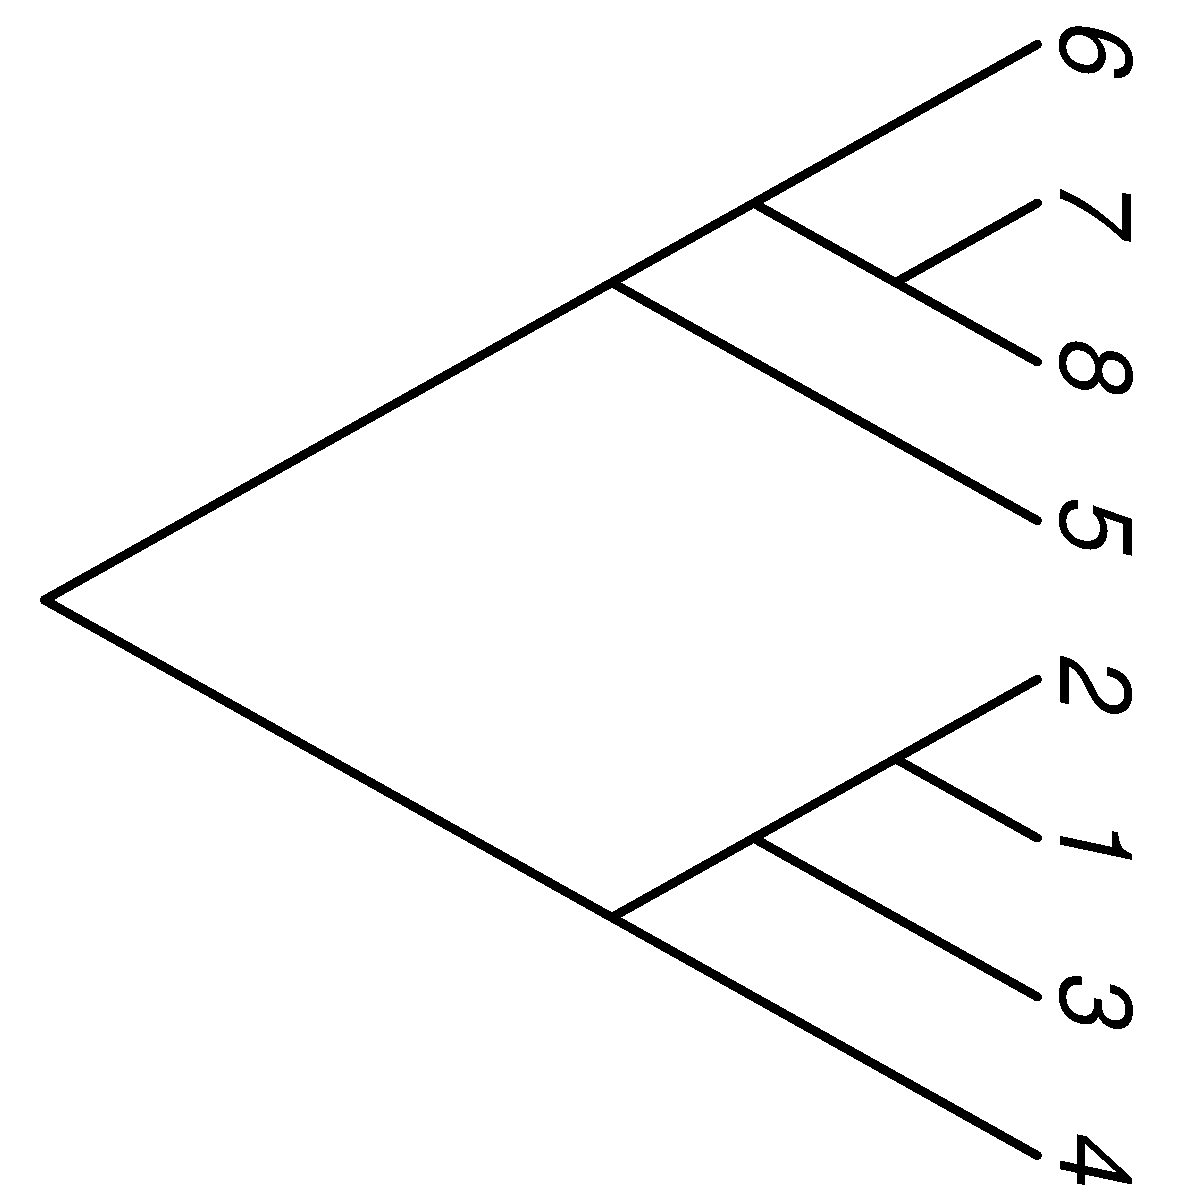
\includegraphics[width=\linewidth]{gatk_tree_rightwards.pdf}
\column{.5\linewidth}
	\begin{center}
	True Tree
	\end{center}
	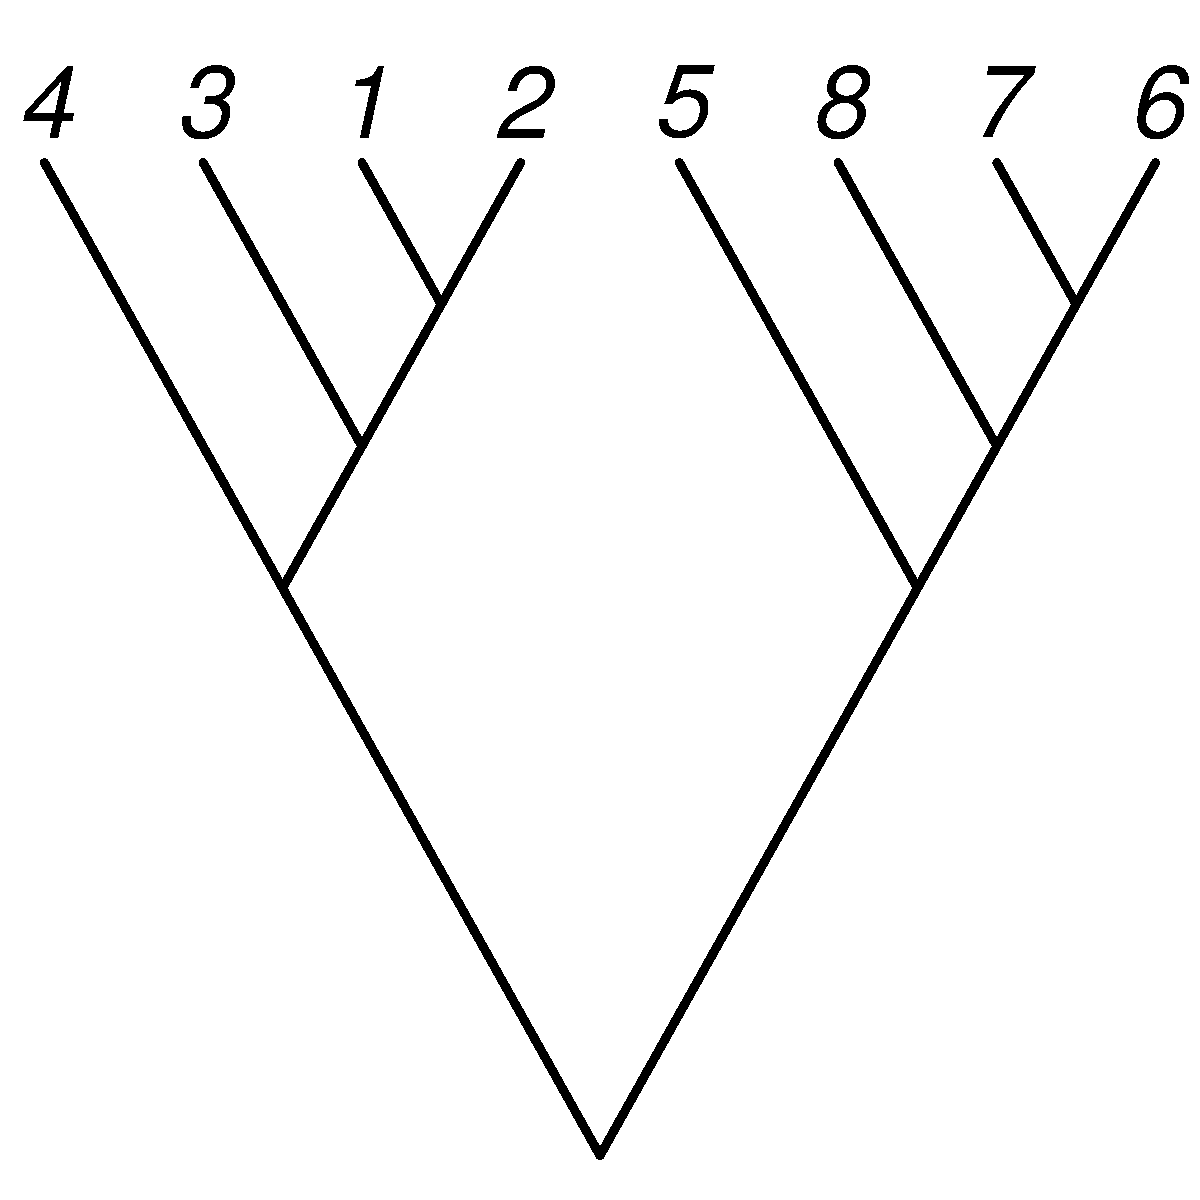
\includegraphics[width=\linewidth,angle=90]{true_tree.pdf}
\end{columns}
\end{frame}

\begin{frame}{Most Reads Are Not Mapped to the \textit{E. grandis} Reference}
\begin{center}
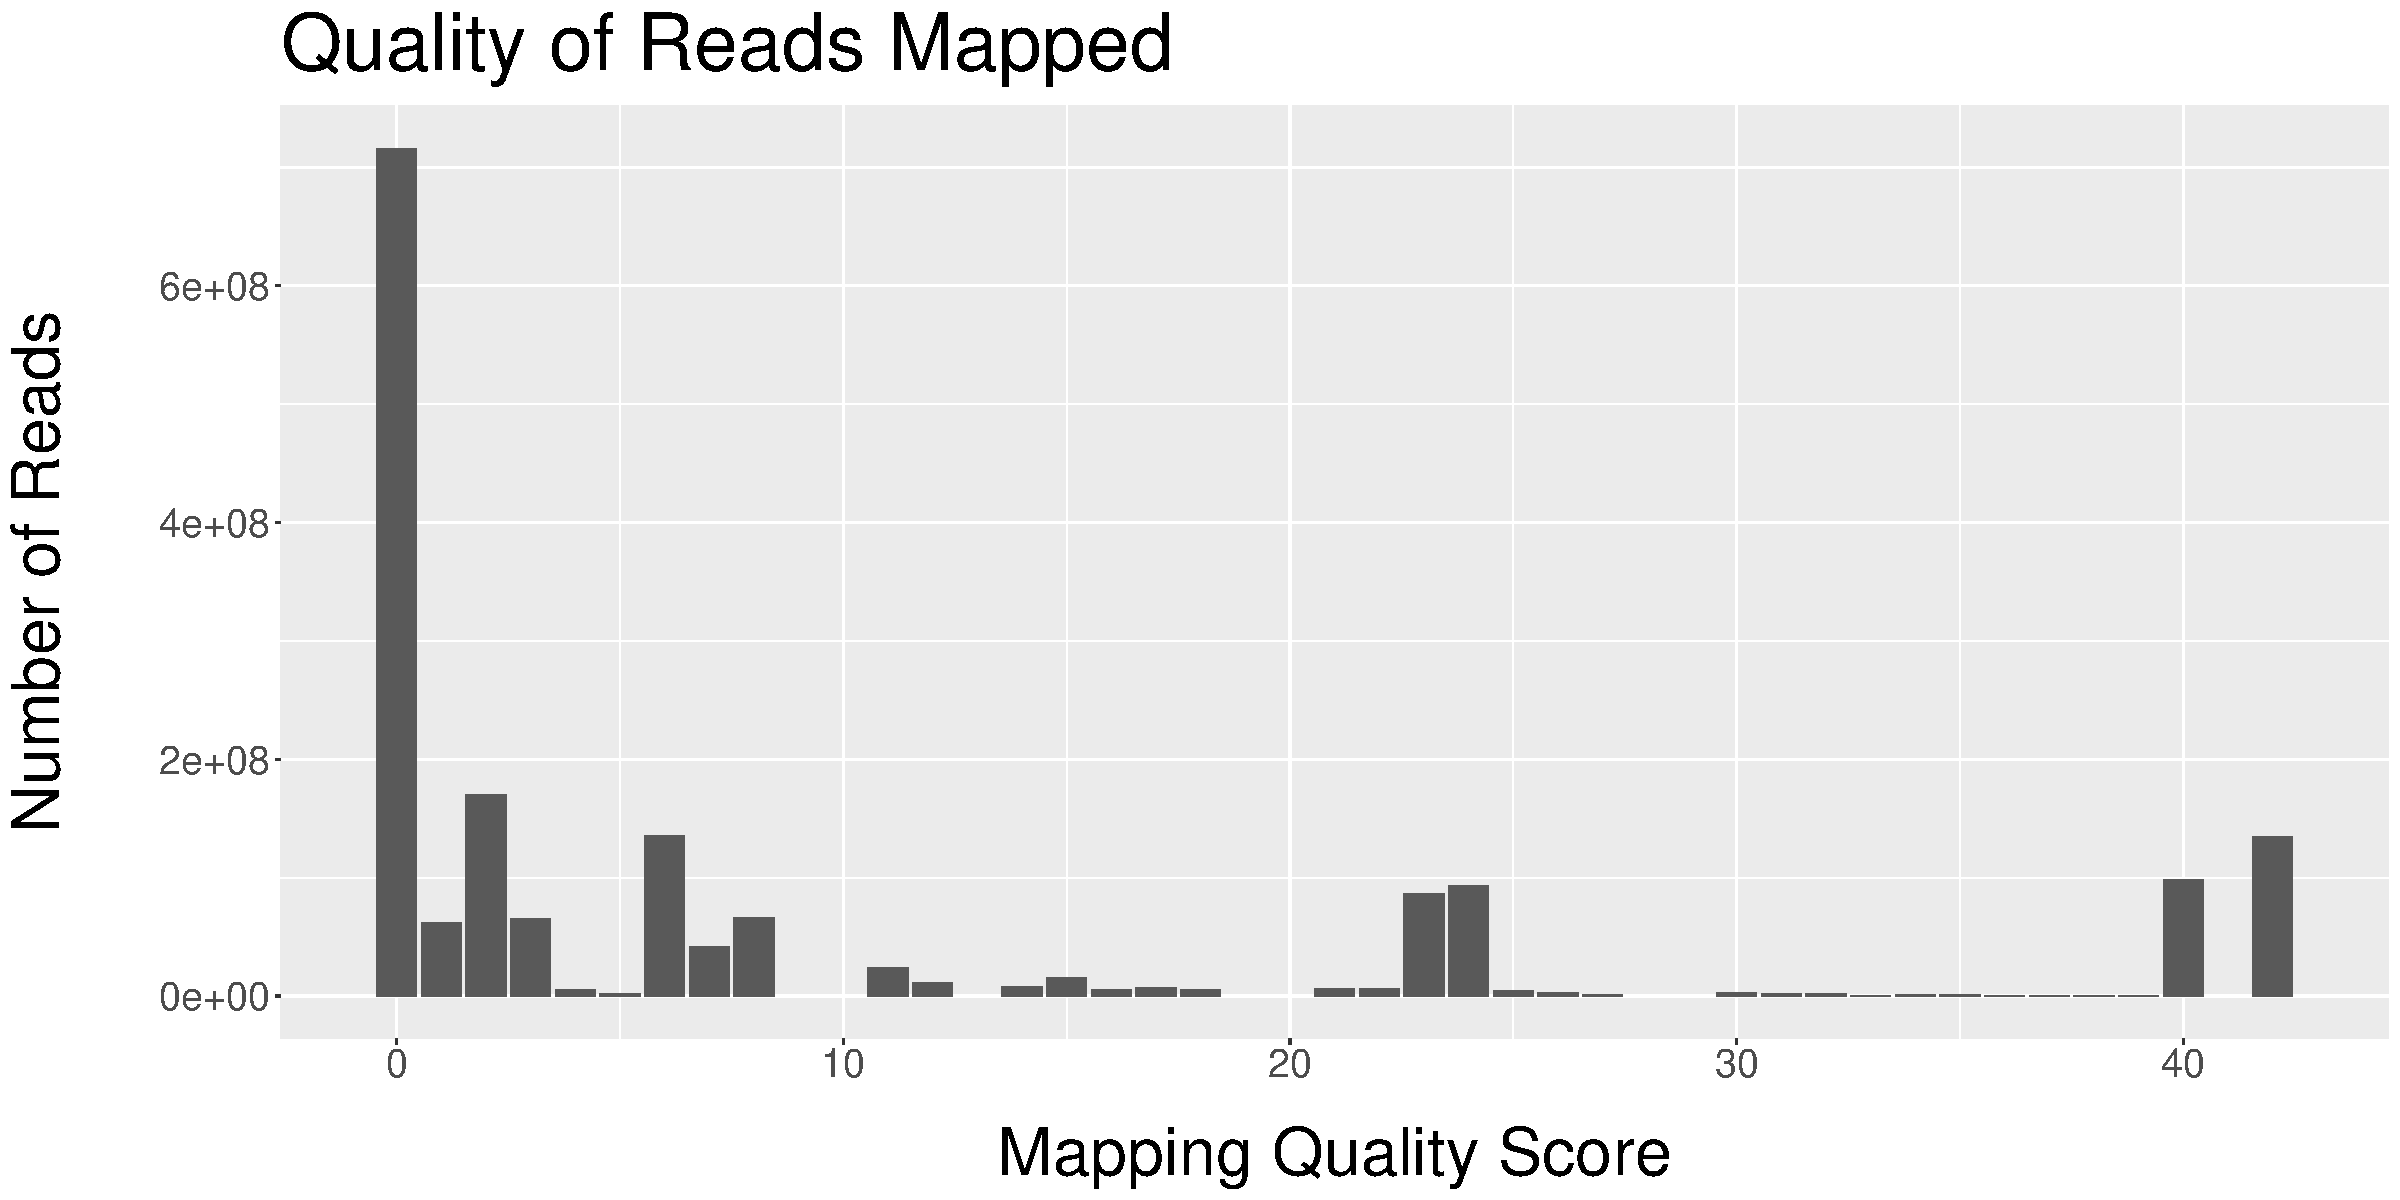
\includegraphics[width=\linewidth]{bowtie1_hist.pdf}
\end{center}
\end{frame}

\begin{frame}{A Reference-Free Method Performs Similarly}
	\begin{columns}
	\column{.5\linewidth}
		\begin{center}
		DiscoSNP++ Tree
		\end{center}
		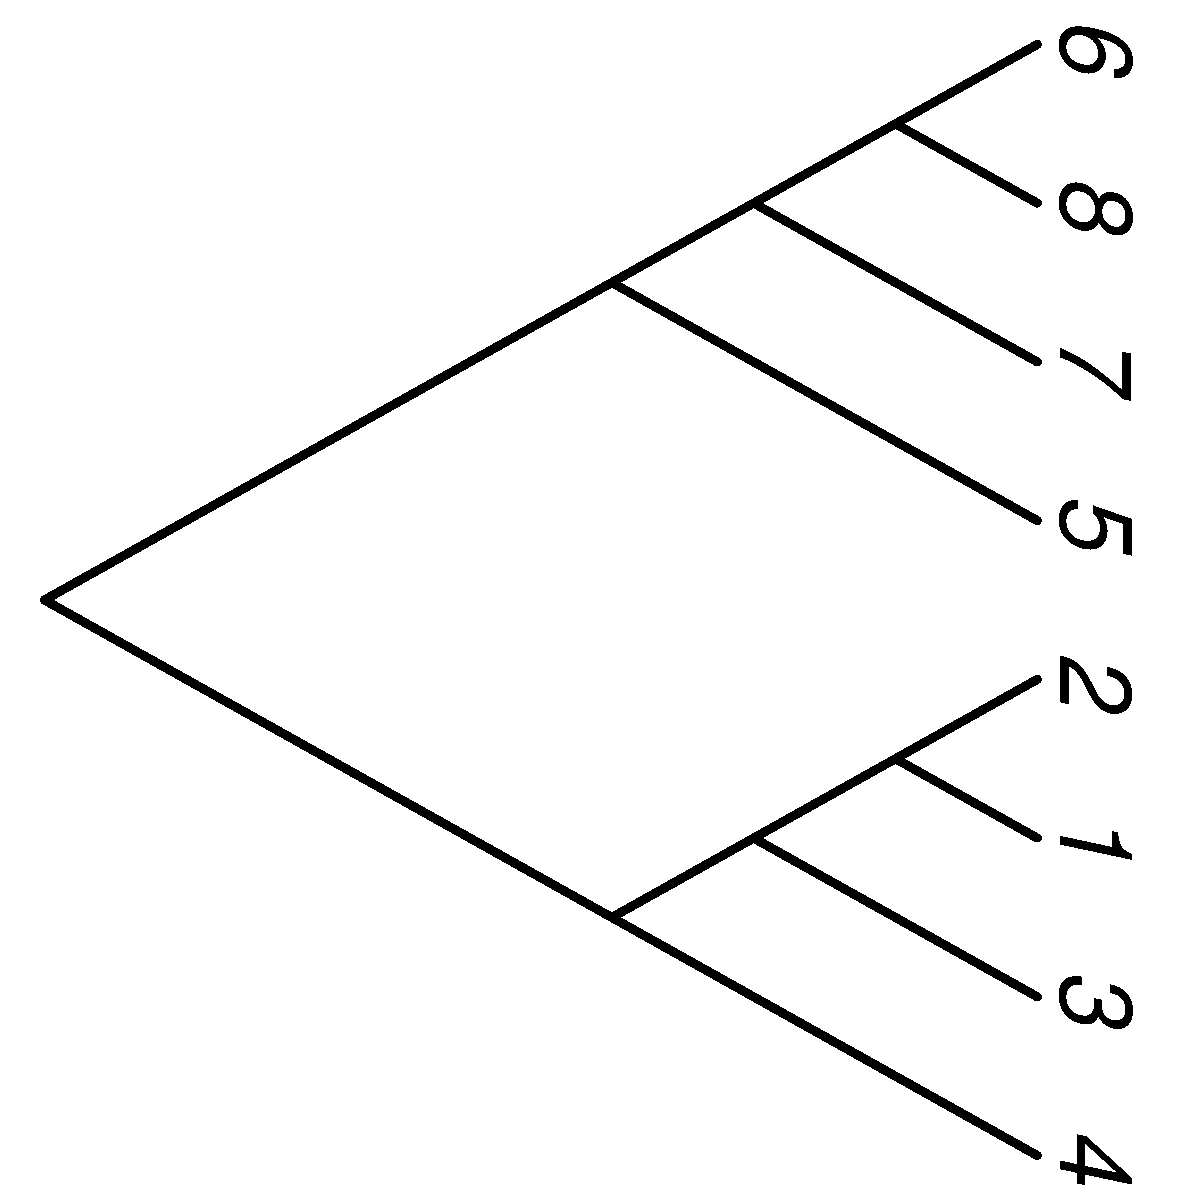
\includegraphics[width=\linewidth]{disco_tree_rightwards.pdf}
	\column{.5\linewidth}
		\begin{center}
		True Tree
		\end{center}
		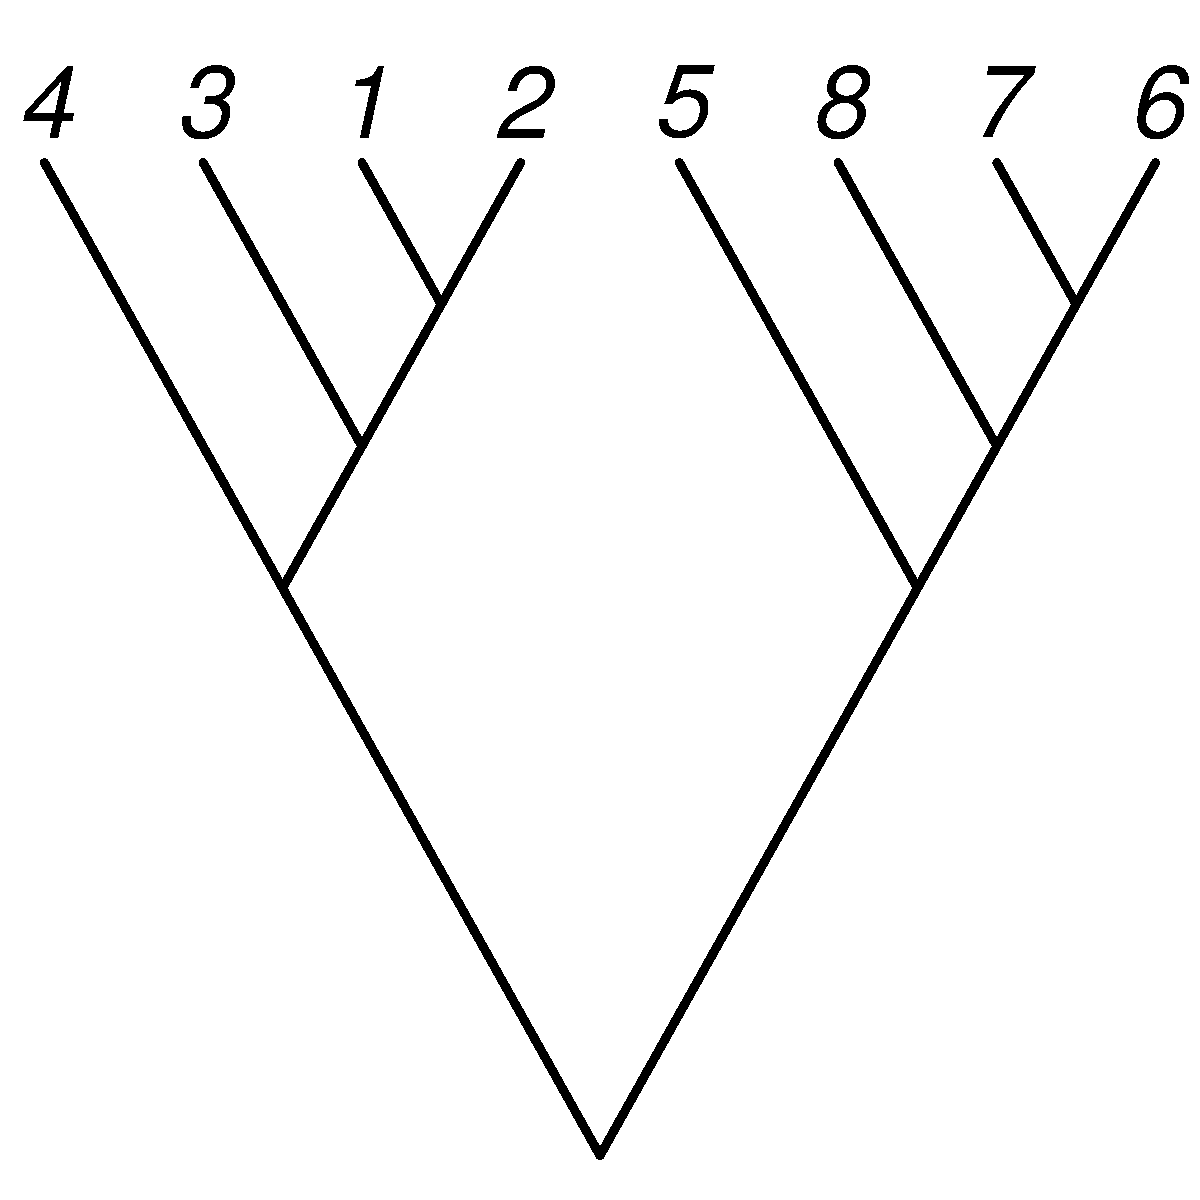
\includegraphics[width=\linewidth,angle=90]{true_tree.pdf}
	\end{columns}
\end{frame}

% \begin{frame}{The Genome Analysis Toolkit}
% 	\begin{itemize}
% 	\item Used a traditional variant-calling pipeline: GATK best practices workflow
% 	\item Reference genome of a close relative: \textit{Eucalyptus Grandis}
% 	\end{itemize}
% 	\begin{columns}
% 	\column{.5\linewidth}
% 		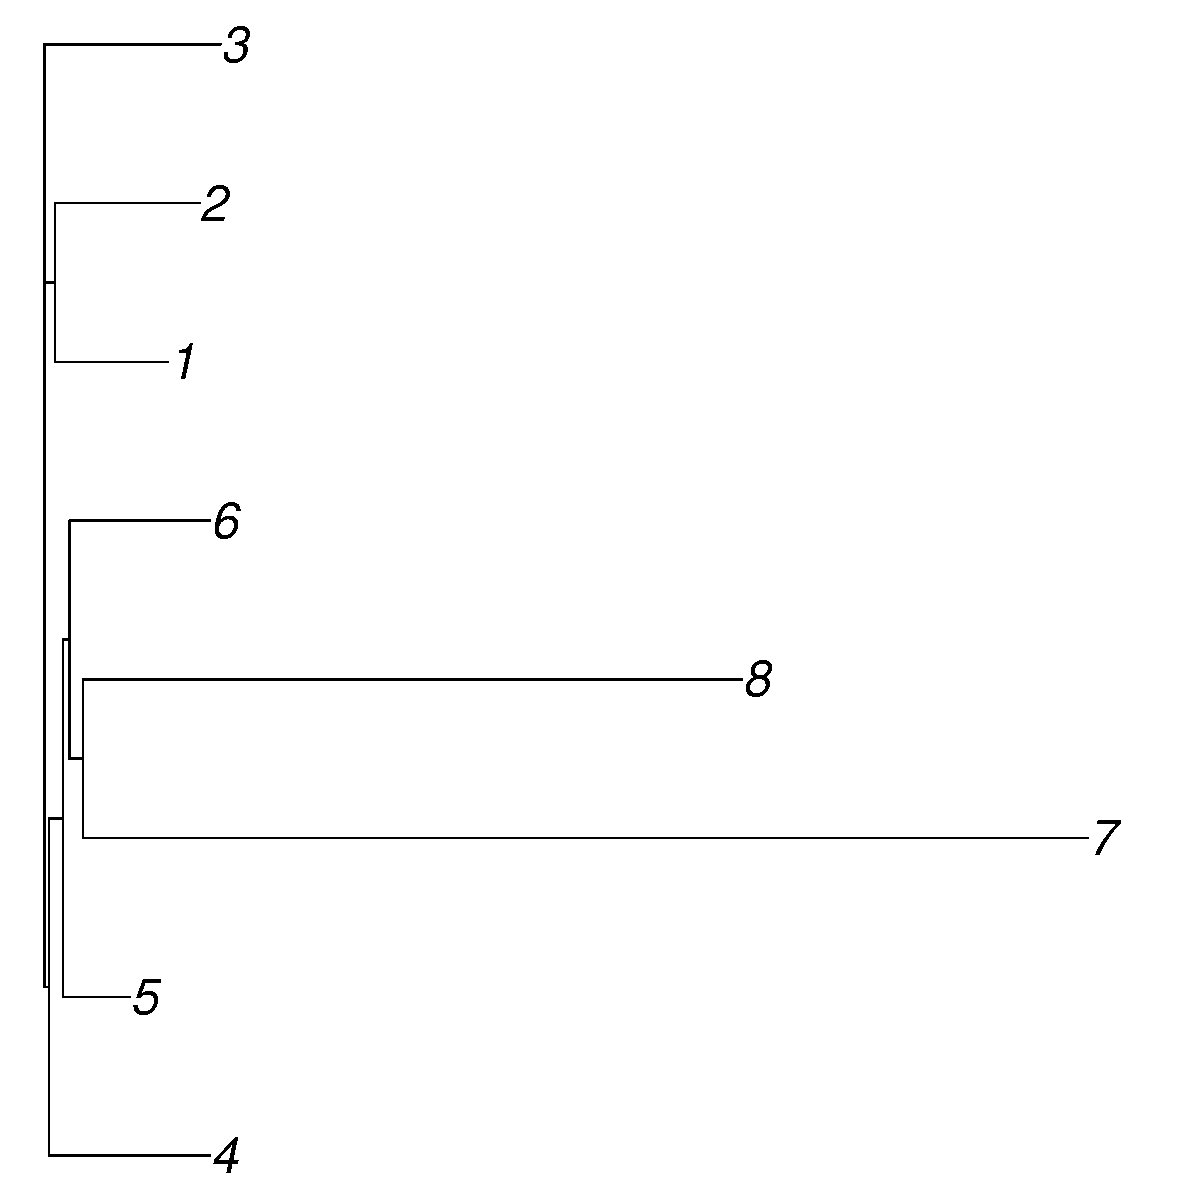
\includegraphics[width=\linewidth]{gatk_tree2.pdf}
% 	\column{.5\linewidth}
% 		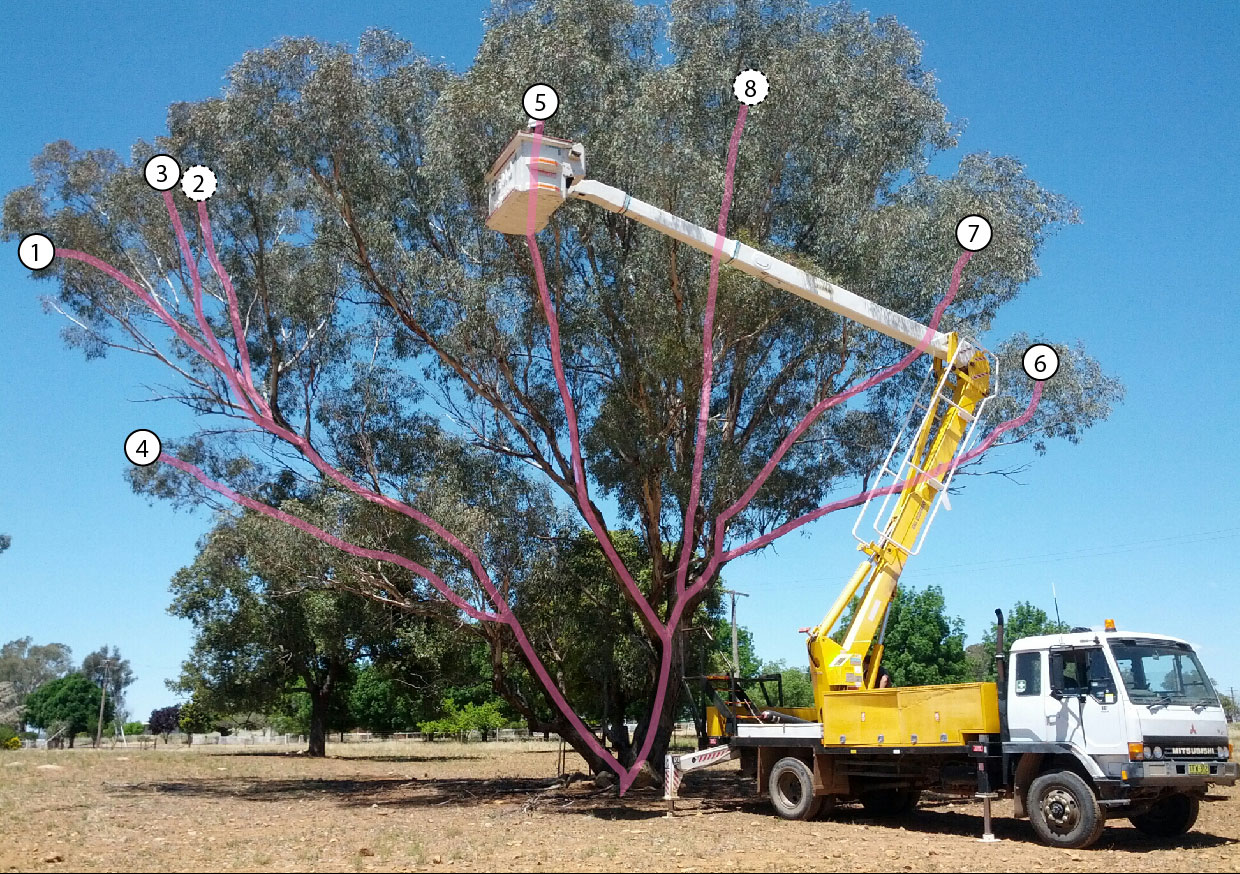
\includegraphics[width=\linewidth]{labeled_tree.jpg}
% 	\end{columns}
% \end{frame}

% \begin{frame}{Branch 7}
% Branch 7 is consistently in the wrong place. Why? What's going on with that branch?
% \begin{definition}
% 	\textbf{Long Branch Attraction} is the tendency of long branches to cluster in a phylogenetic tree
% \end{definition}

% \begin{itemize}
% \item Branch 7 is the longest branch
% \item May be affected by assumptions about zygosity
% \item Do particular genomic regions make mutation calling more difficult for one method?
% \end{itemize}
% \end{frame}

\begin{frame}{Improving Alignment}
	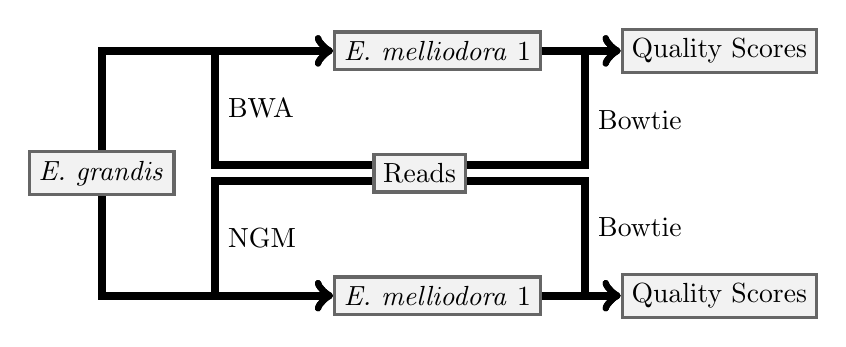
\begin{tikzpicture}[align=center,cnode/.style={rectangle,draw=black!60,fill=black!5,very thick}, node distance = 1cm and 1cm]
		\node[cnode] (eg){\textit{E. grandis}};
		\node[cnode,minimum width=1cm] (reads)[right = 2.5cm of eg]{Reads};
		\node[cnode] (em1)[above right = 1cm and 2cm of eg]{\textit{E. melliodora} 1};
		\node[cnode] (em2)[below right = 1cm and 2cm of eg]{\textit{E. melliodora} 1};
		\node[cnode] (bwaq)[right = 1cm of em1]{Quality Scores};
		\node[cnode] (ngmq)[right = 1cm of em2]{Quality Scores};
		\draw[line width=1mm,->] (eg.north) |- (em1);
		\draw[line width=1mm,->] (eg.south) |- (em2);
		% \draw[line width=3mm,->] ($(reads.west)+(0cm,.5cm)$) to[out=180,in=180] ($(em1.west)-(1.5cm,0cm)$) -- (em1.west);
		\draw[line width=1mm,->] ($(reads.west)+(0cm,.1cm)$) -- ++(-2cm,0cm) |- (em1.west) node[pos=.25,right]{BWA};
		\draw[line width=1mm,->] ($(reads.west)-(0cm,.1cm)$) -- ++(-2cm,0cm) |- (em2.west) node[pos=.25,right]{NGM};
		\draw[line width=1mm,->] (em1) -- (bwaq);
		\draw[line width=1mm,->] (em2) -- (ngmq);
		\draw[line width=1mm,->] ($(reads.east)+(0cm,.1cm)$) -- ++(1.5cm,0cm) |- (bwaq.west) node[pos=.2,right]{Bowtie};
		\draw[line width=1mm,->] ($(reads.east)-(0cm,.1cm)$) -- ++(1.5cm,0cm) |- (ngmq.west) node[pos=.2,right]{Bowtie};
	\end{tikzpicture}
\end{frame}


\begin{frame}{The Choice of Aligner Impacts Mapping Quality}
\begin{center}
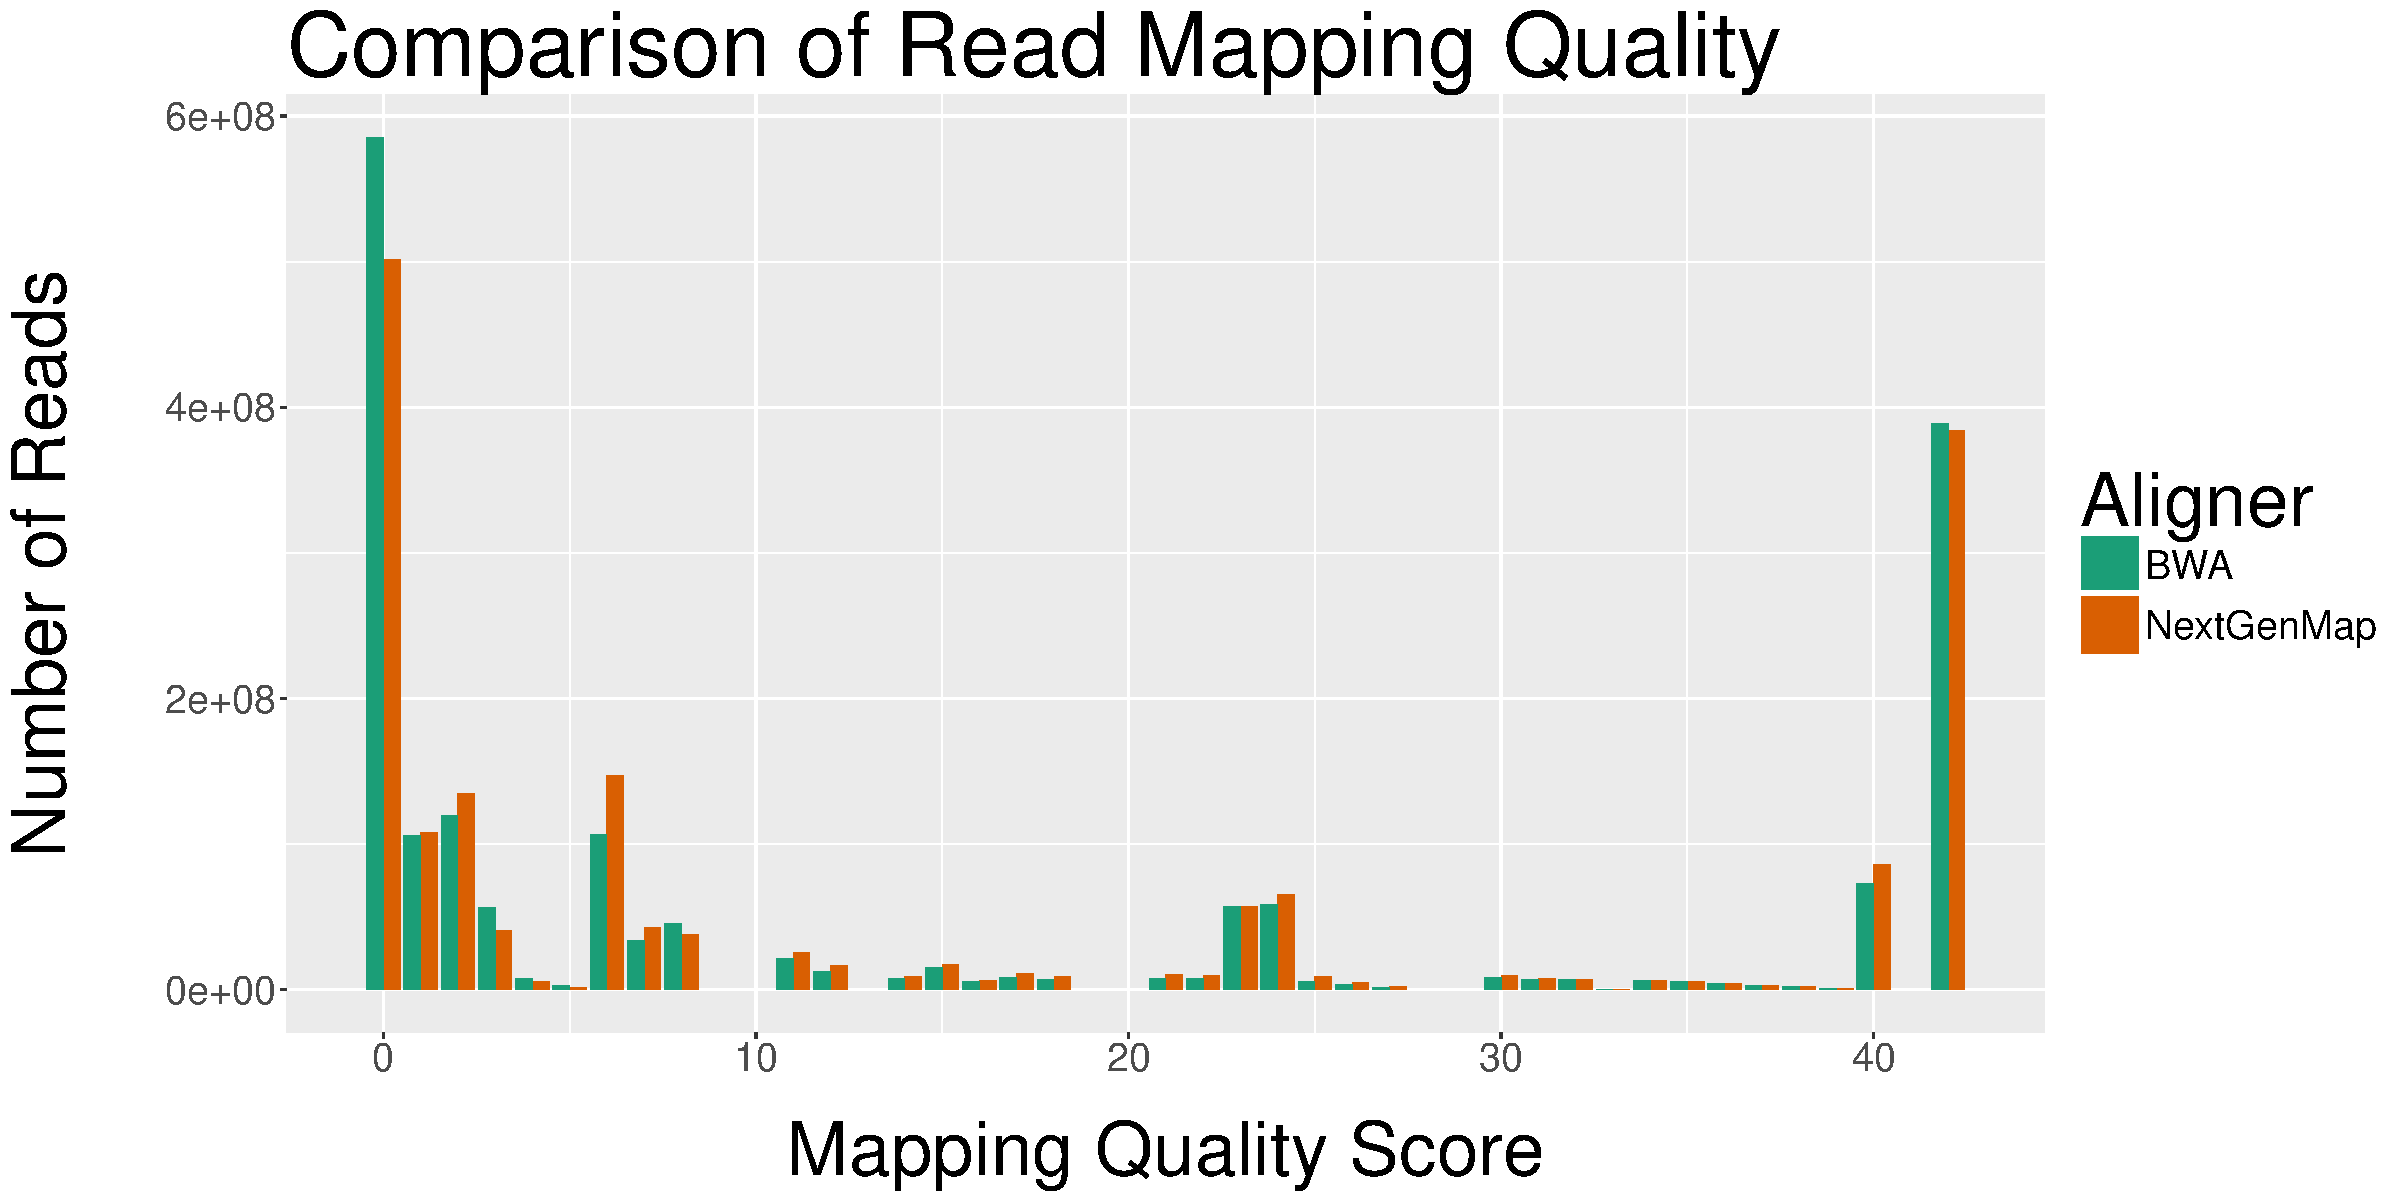
\includegraphics[width=.95\linewidth]{aligner_comparison_hist.pdf}
\end{center}
\end{frame}


\begin{frame}{If you want something done right...}

Use \textit{E. melliodora} genome as a starting place, then generate a new reference and map to that reference.

\begin{center}
	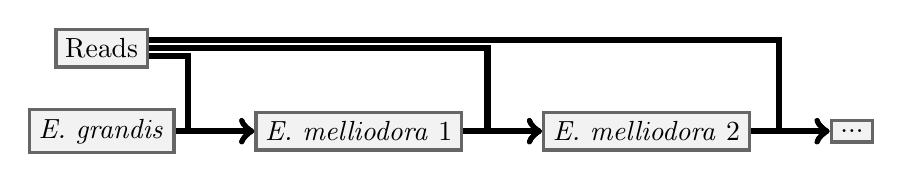
\begin{tikzpicture}[cnode/.style={rectangle,draw=black!60,fill=black!5,very thick}, node distance = 1 cm]
		\node[cnode] (reads){Reads};
		\node[cnode] (eg)[below = .5cm of reads]{\textit{E. grandis}};
		\node[cnode] (em1)[right = of eg]{\textit{E. melliodora} 1};
		\node[cnode] (em2)[right = of em1]{\textit{E. melliodora} 2};
		\node[cnode] (etc)[right = of em2] {...};
		\draw[line width=.8mm,->] ($(reads.east)-(0cm,.1cm)$) -- ($(reads.east)+(.5cm,-.1cm)$) |- (em1.west);
		\draw[line width=.8mm,->] (reads.east) -- ($(reads.east)+(4.3cm,0cm)$) |- (em2.west);
		\draw[line width=.8mm,->] ($(reads.east)+(0cm,.1cm)$) -- ($(reads.east)+(8cm,.1cm)$) |- (etc.west);
		\draw[line width=.8mm,->] (eg) -- (em1);
		\draw[line width=.8mm,->] (em1) -- (em2);
		\draw[line width=.8mm,->] (em2) -- (etc);
	\end{tikzpicture}
\end{center}

% \begin{alertblock}{Next Steps}
% \begin{itemize}
% \item Generate a genome and recursively improve it with multiple tools
% \item Filter repetitive elements that complicate mapping
% \item How do the mutations found with DiscoSNP compare to those found with GATK? Is there a pattern?
% \item Validation
% \end{itemize}
% \end{alertblock}

\end{frame}

\begin{frame}{Our New Reference Improves Mapping Quality}
\begin{center}
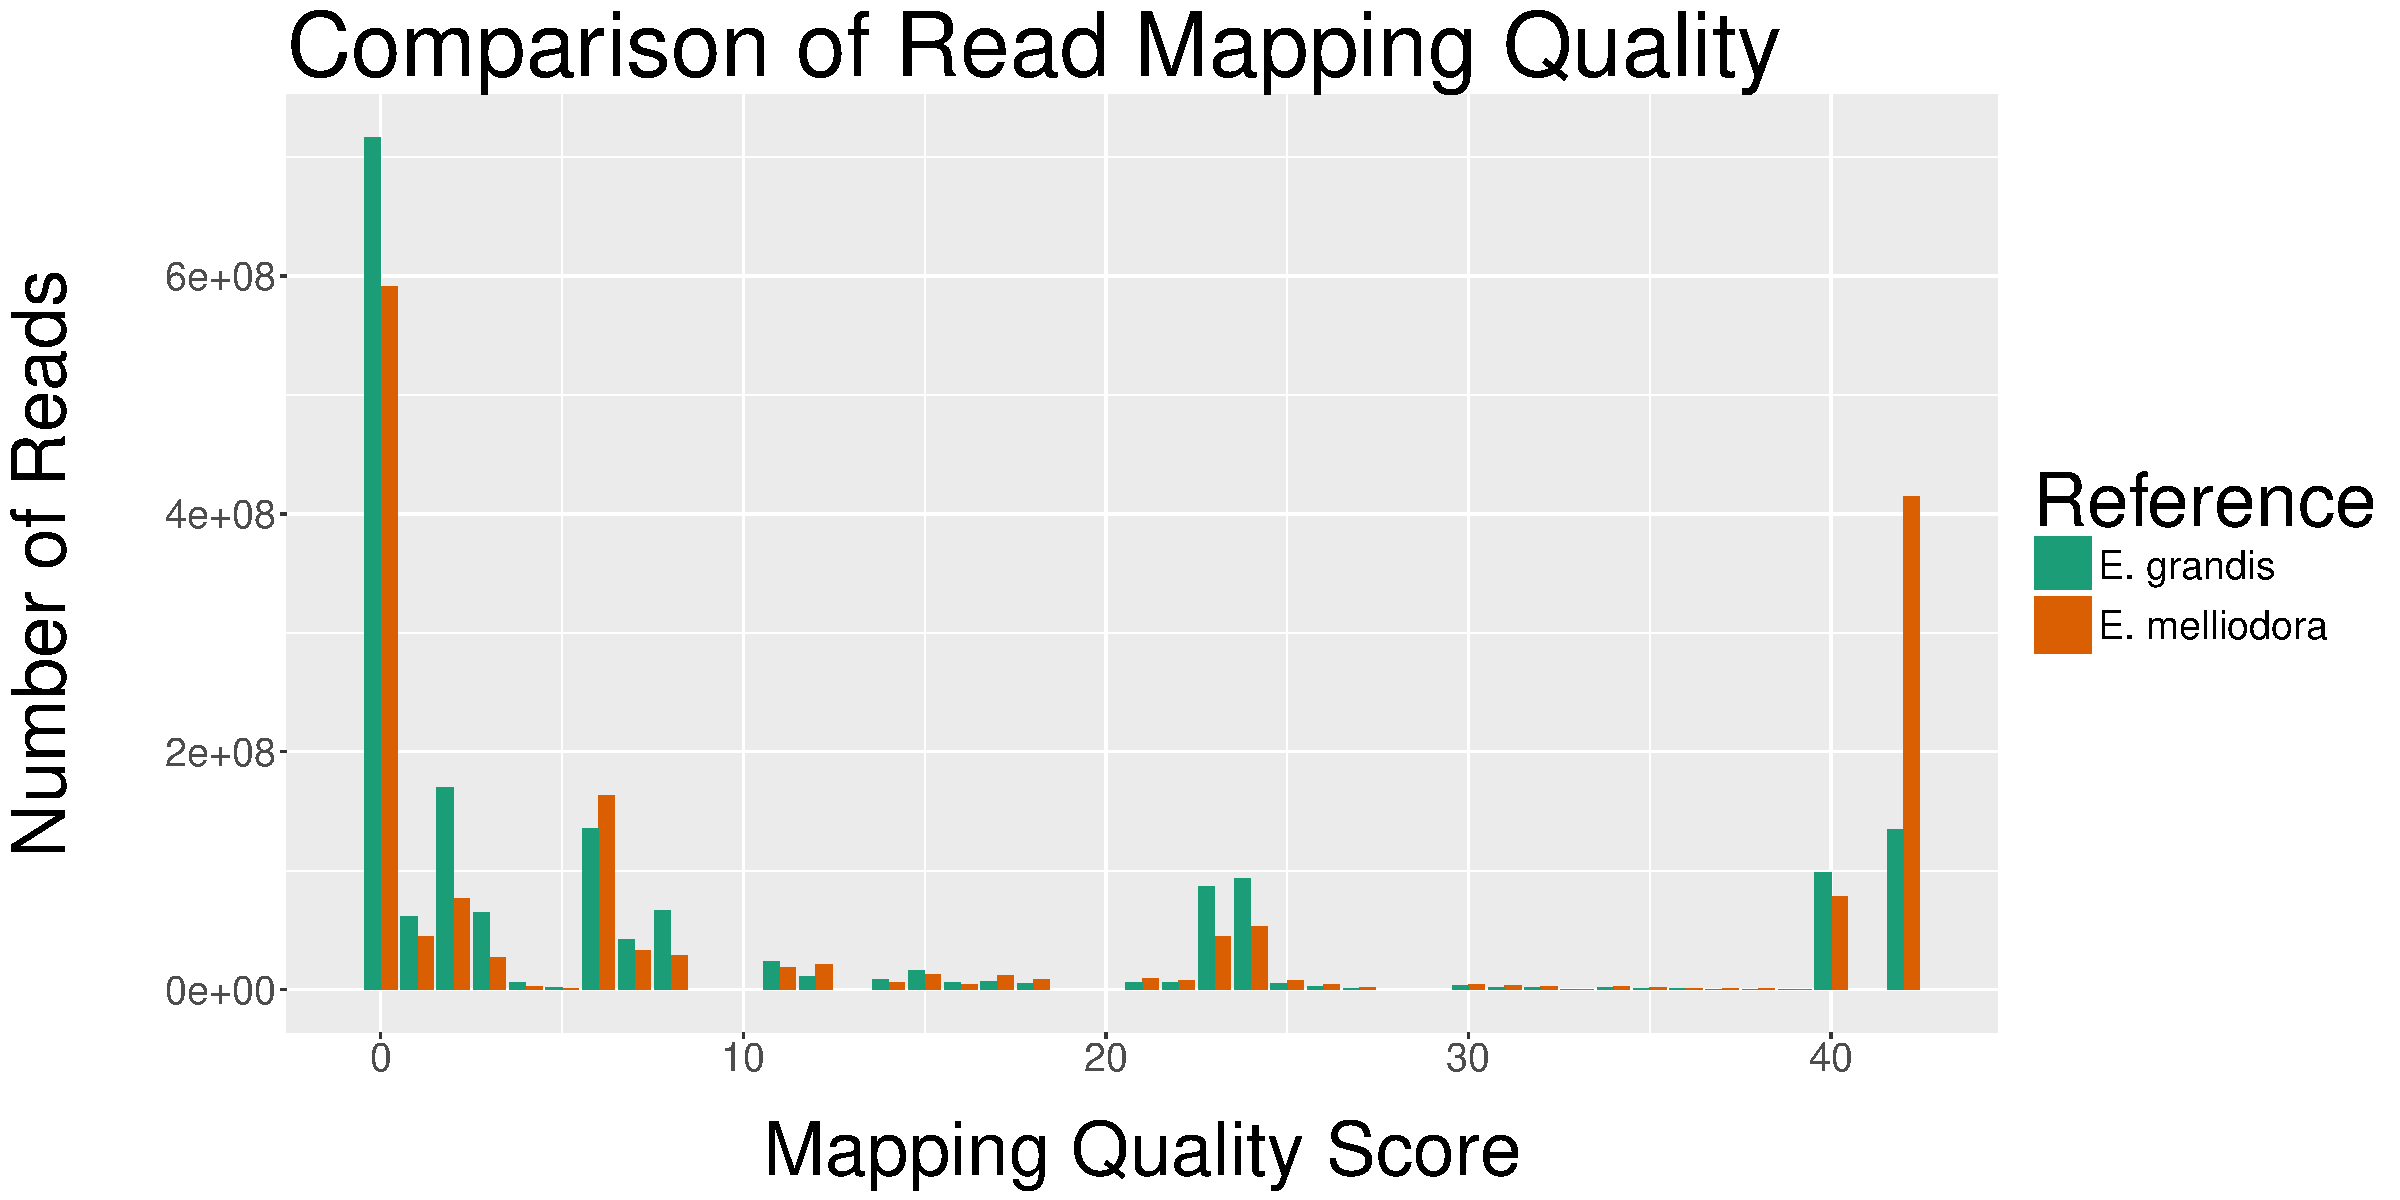
\includegraphics[width=.95\linewidth]{both_hist.pdf}
\end{center}
\end{frame}





\begin{frame}{Next Steps}
\begin{itemize}
\item Iterate to improve the reference we've created.
\item Filter out repetitive elements that make mapping difficult
\item Error correct reads
\end{itemize}
\end{frame}

\begin{frame}{Dissertation Ideas}
\begin{itemize}
\item Create variant caller able to utilize error models from diverse sequencing platforms
\item GATK Base-Quality Score Recalibration-like process without need for alignment and truth-set variant calls
\item Study error correction impact on alignment and variant calling
\end{itemize}
\end{frame}

\end{document}